\section{Inwentaryzacja sprzętu i infrastruktury dostępnej w przedsiębiorstwie}
\subsection{Budynki}
\paragraph{}
Firma ma swoją siedzibę w dwóch budynkach oddalonych od siebie o około 50m. Pierwsza z budowli składa się z czterech pieter, natomiast druga z trzech. Pięć kondygnacji jest zaadaptowanych jako pomieszczenia dla programistów. Dwie kondygnacja przeznaczone są na serwerownie, pomieszczenia administracyjne i  pomieszczenia członków zarządu. Na każdym piętrze zlokalizowana będzie sala konferencyjna, oraz kuchnia i pomieszczenia sanitarne.
\paragraph{}
\subsubsection{Budynek 1}
\paragraph{}
Na parterze mieści się serwerownia i pomieszczenia pracowników administracyjnych. Kolejne dwie kondygnacje zajmują programiści aplikacji webowych, a na ostatnim piętrze mają swoją siedzibę programiści aplikacji na systemy mobilne.

\subsubsection{Budynek 2}
\paragraph{}
Parter oraz pierwsze piętro zajmują sale konferencyjne oraz pomieszczenia dla programistów. Na ostatnim piętrze znajdują się biura członków zarządu.

\paragraph{}
Poniżej znajdują się plany obu budynków w skali $1:265$ oraz ich wzajemne położenie.

\begin{table}[h]
  \begin{center}
      \begin{tabular}{|c|c|}
      \hline
        1       & Sala konferencyjna \\ \hline
        2       & Serwerownia \\ \hline
        3,4,5   & Pomieszczenia administracyjne \\ \hline
        7       & Pomieszczenia programistów \\ \hline
        11      & Pomieszczenia członków zarządu \\ \hline
     \end{tabular}
  \end{center}
  \caption{Oznaczenia pomieszczeń}
\end{table}

\paragraph{}
\paragraph{}
\paragraph{}
\begin{figure}[H]
  \begin{center}
    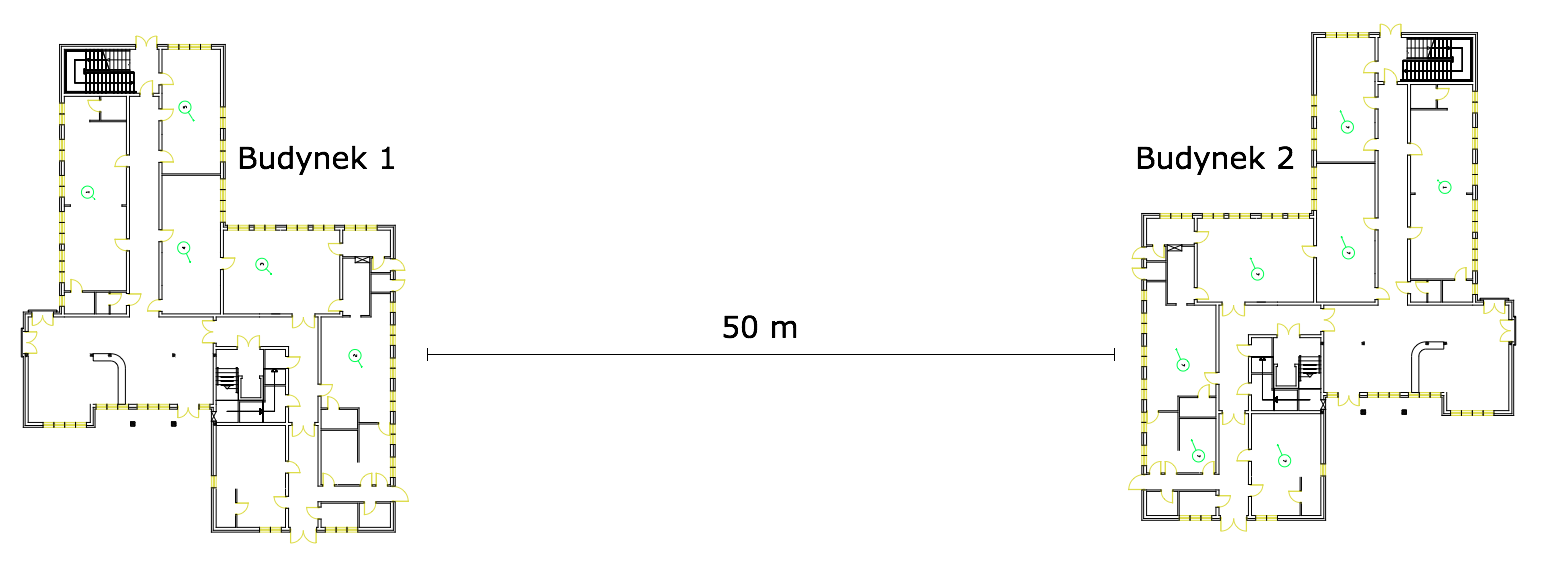
\includegraphics[width=\textwidth]{img/polo.png}
    \caption{Wzajemne położenie budynków}
  \end{center}
\end{figure}


\begin{figure}[H]
  \begin{center}
    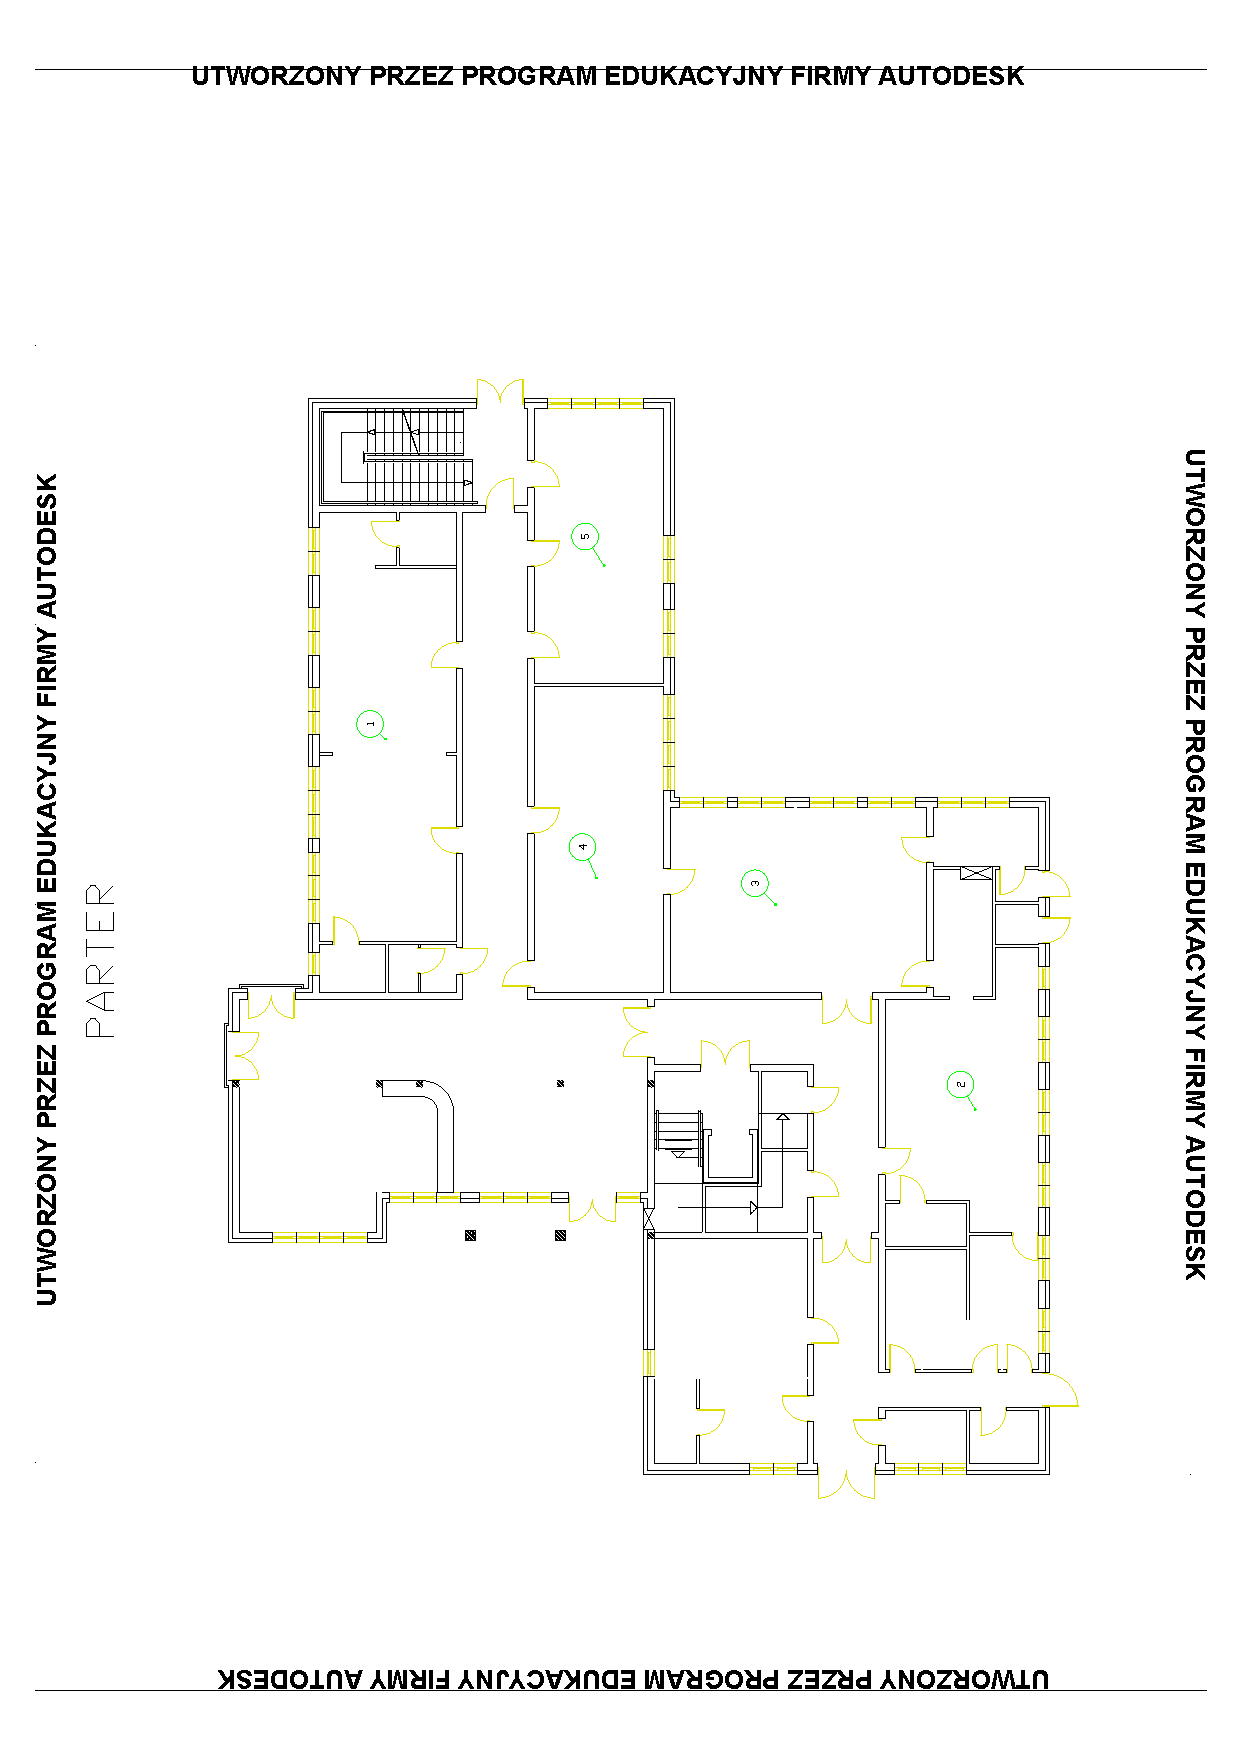
\includegraphics[width=\textwidth]{img/b1-0.pdf}
    \caption{Budynek 1 - Parter}
  \end{center}
\end{figure}

\begin{figure}[H]
  \begin{center}
    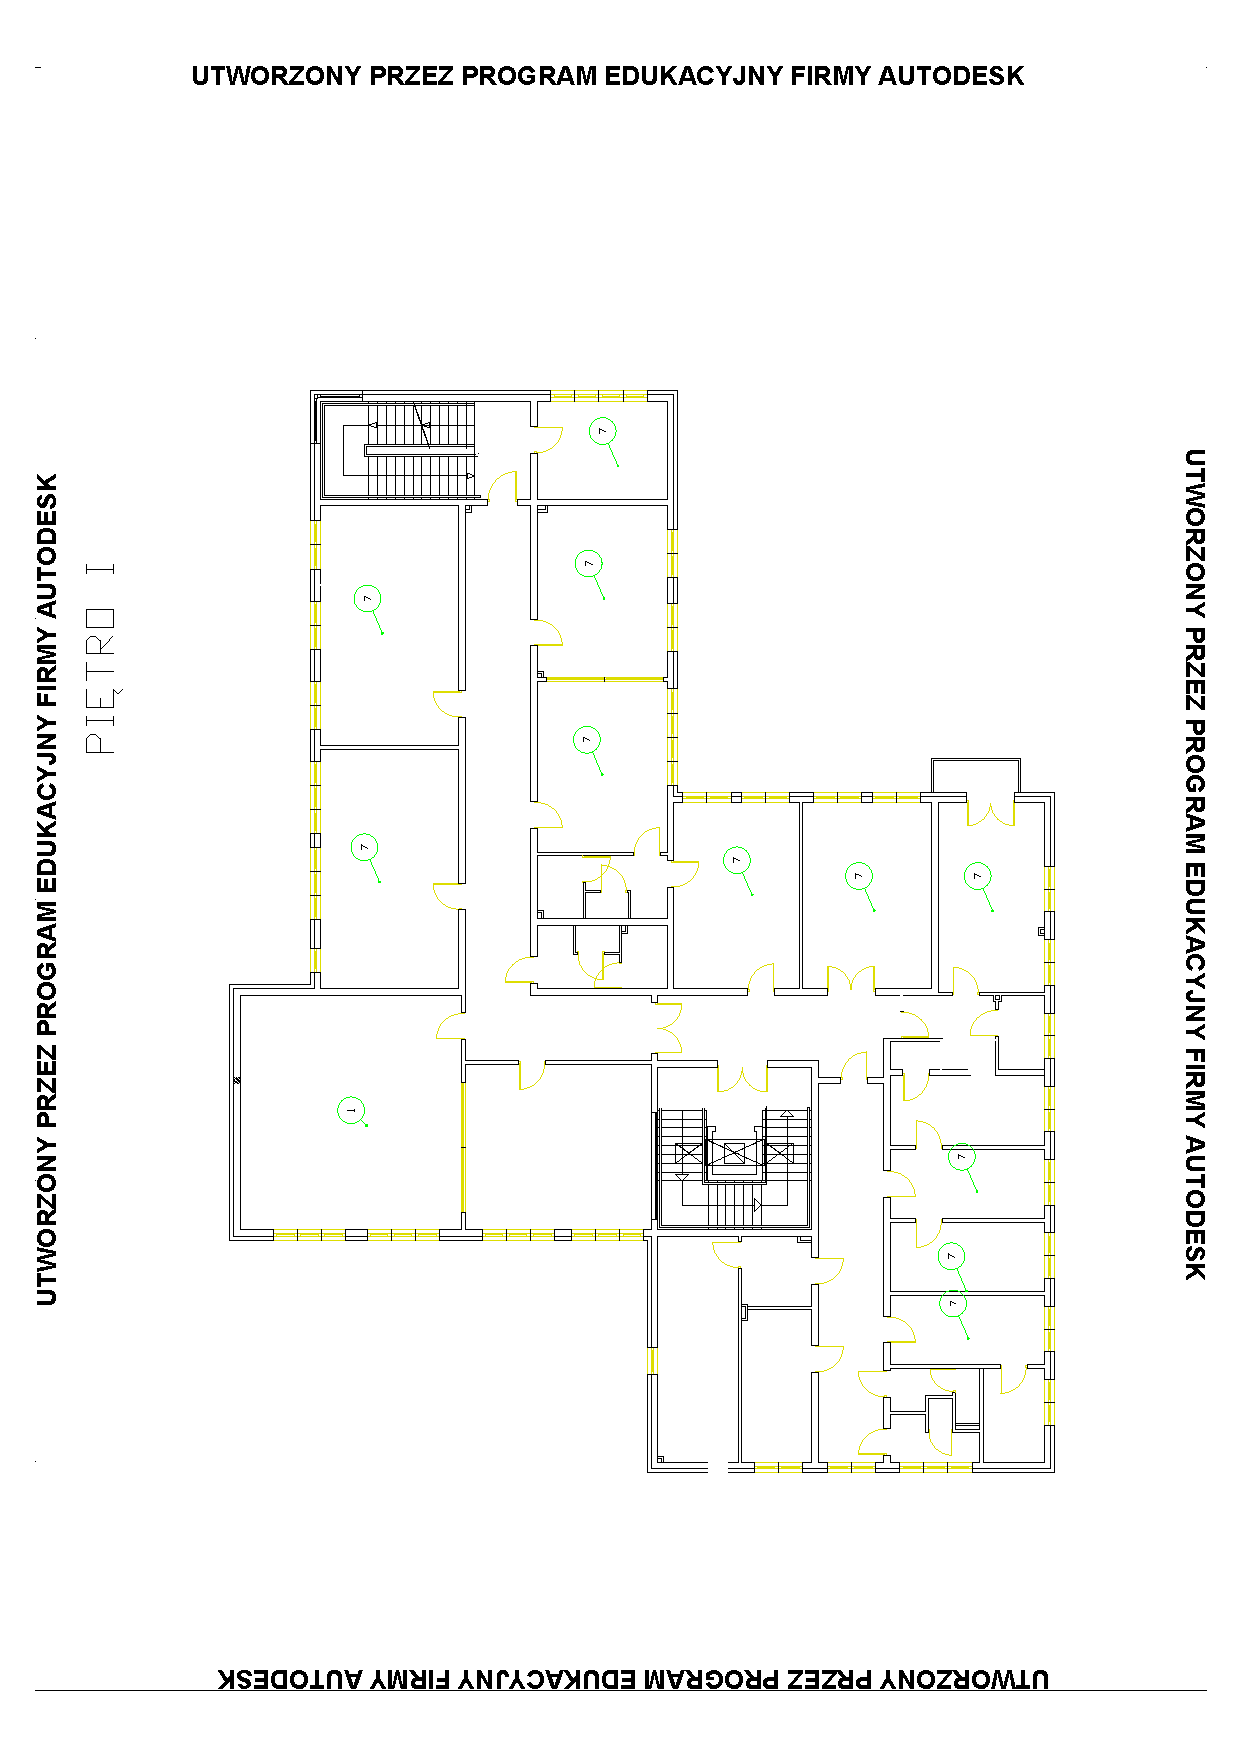
\includegraphics[width=\textwidth]{img/b1-1.pdf}
    \caption{Budynek 1 - Piętro I}
  \end{center}
\end{figure}

\begin{figure}[H]
  \begin{center}
    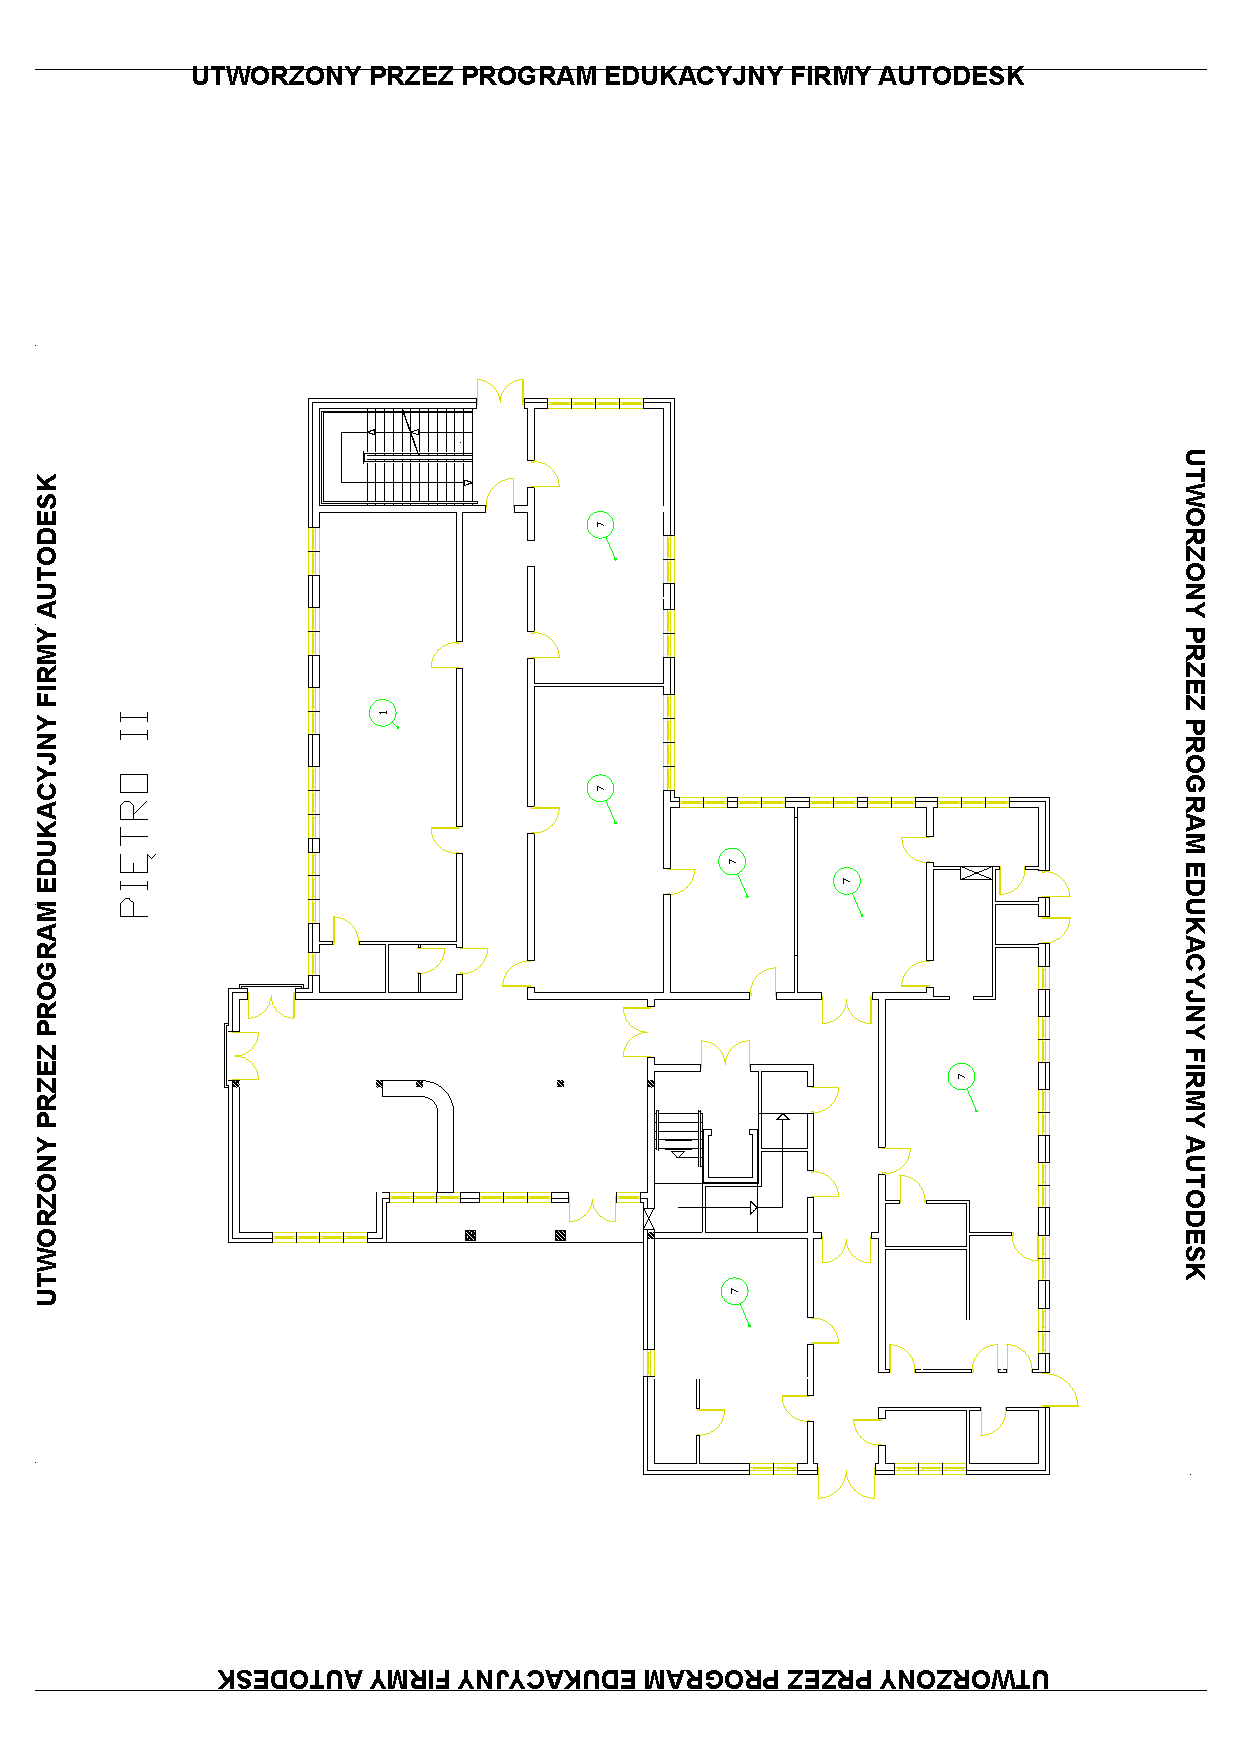
\includegraphics[width=\textwidth]{img/b1-2.pdf}
    \caption{Budynek 1 - Piętro II}
  \end{center}
\end{figure}

\begin{figure}[H]
  \begin{center}
    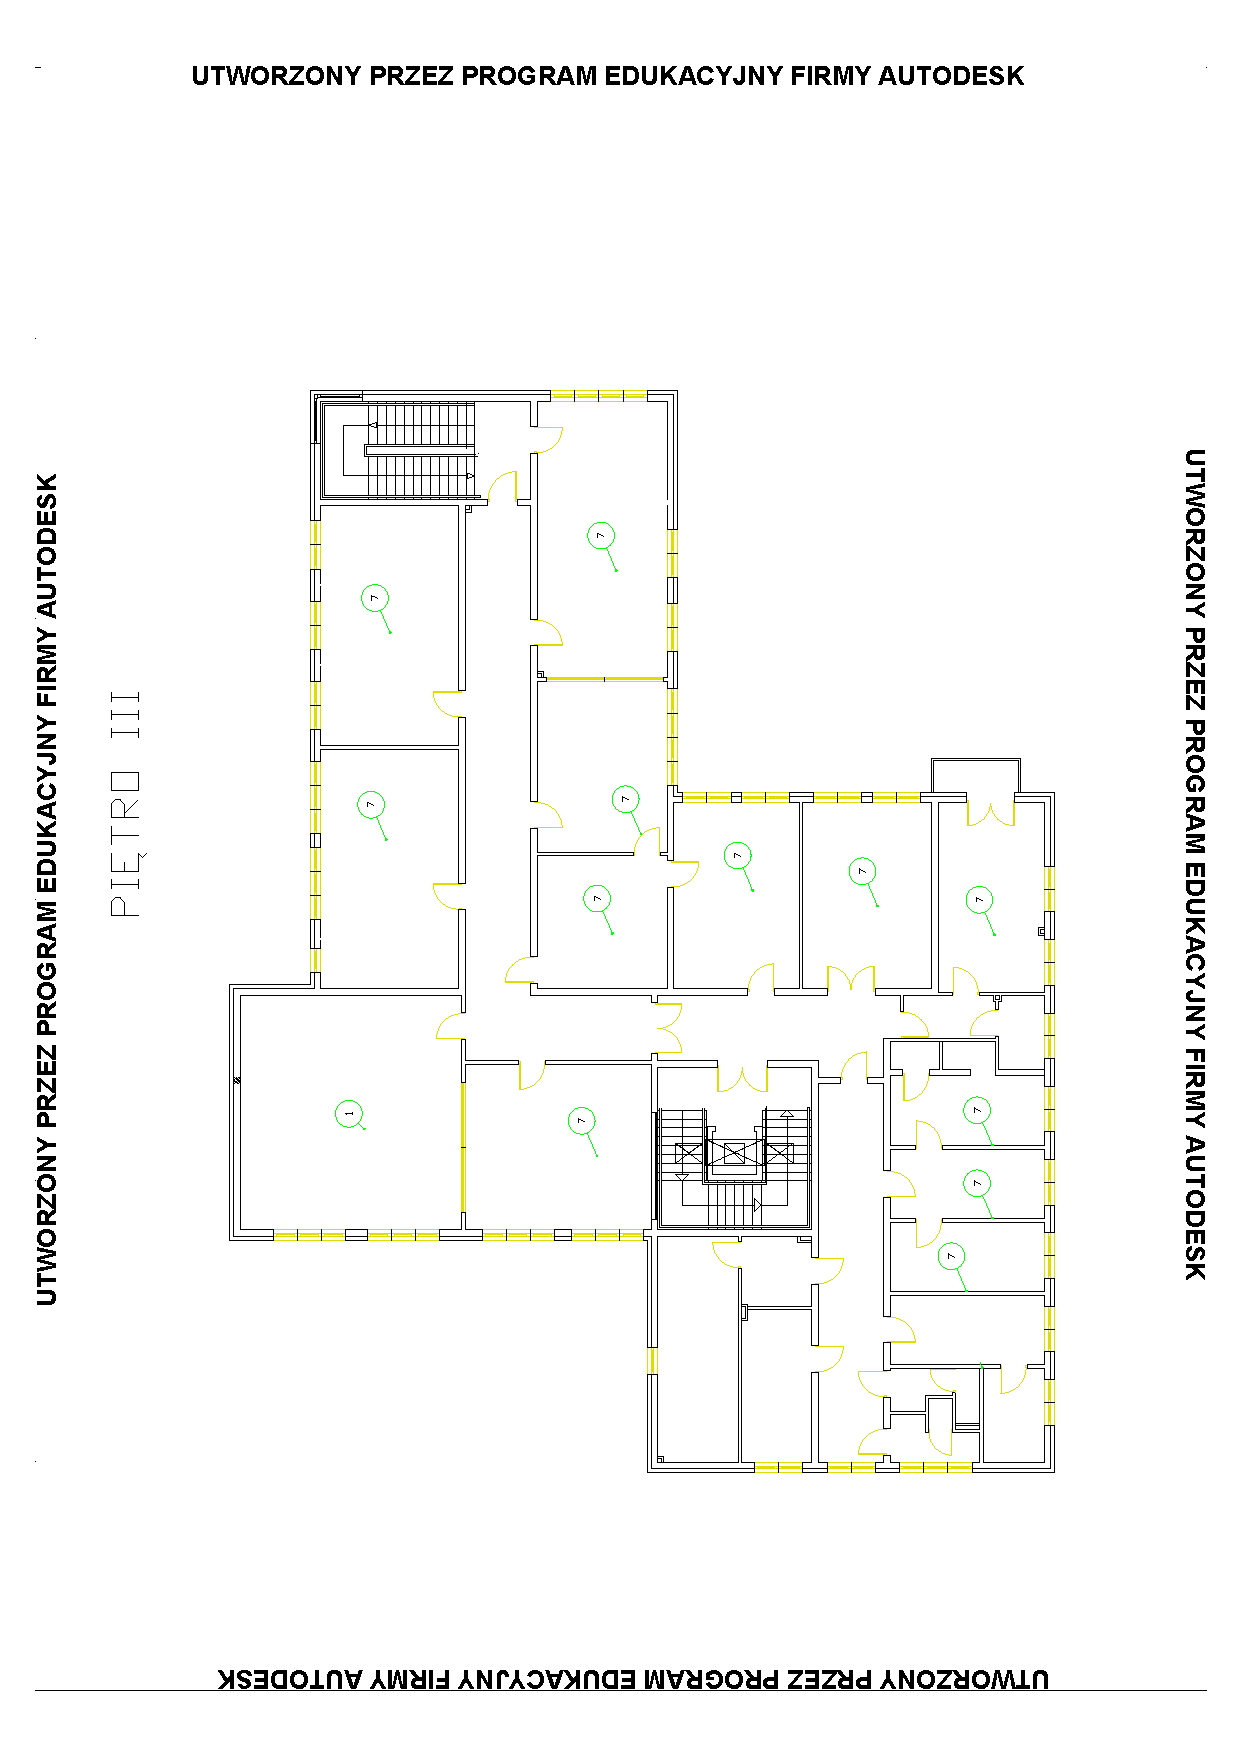
\includegraphics[width=\textwidth]{img/b1-3.pdf}
    \caption{Budynek 1 - Piętro III}
  \end{center}
\end{figure}

\begin{figure}[H]
  \begin{center}
    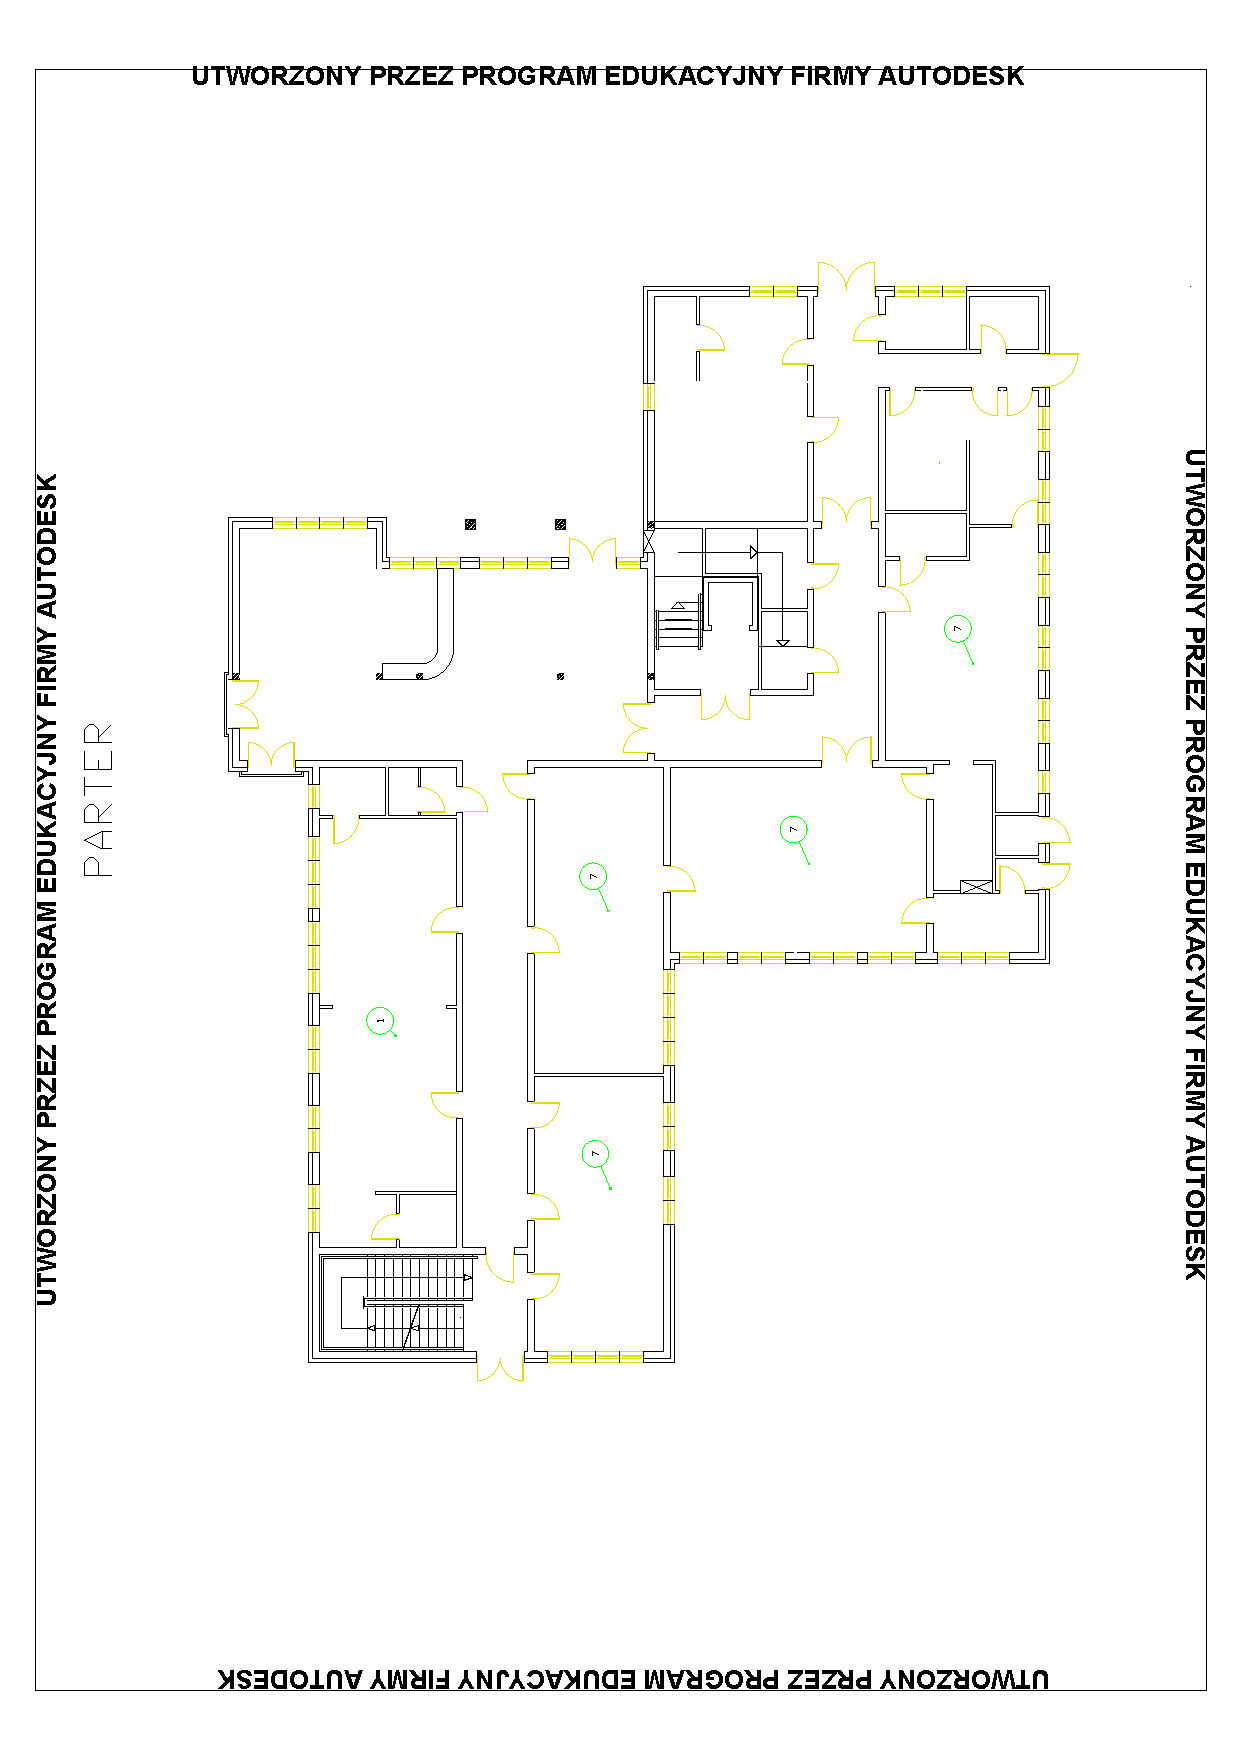
\includegraphics[width=\textwidth]{img/b2-0.pdf}
    \caption{Budynek 2 - Parter}
  \end{center}
\end{figure}

\begin{figure}[H]
  \begin{center}
    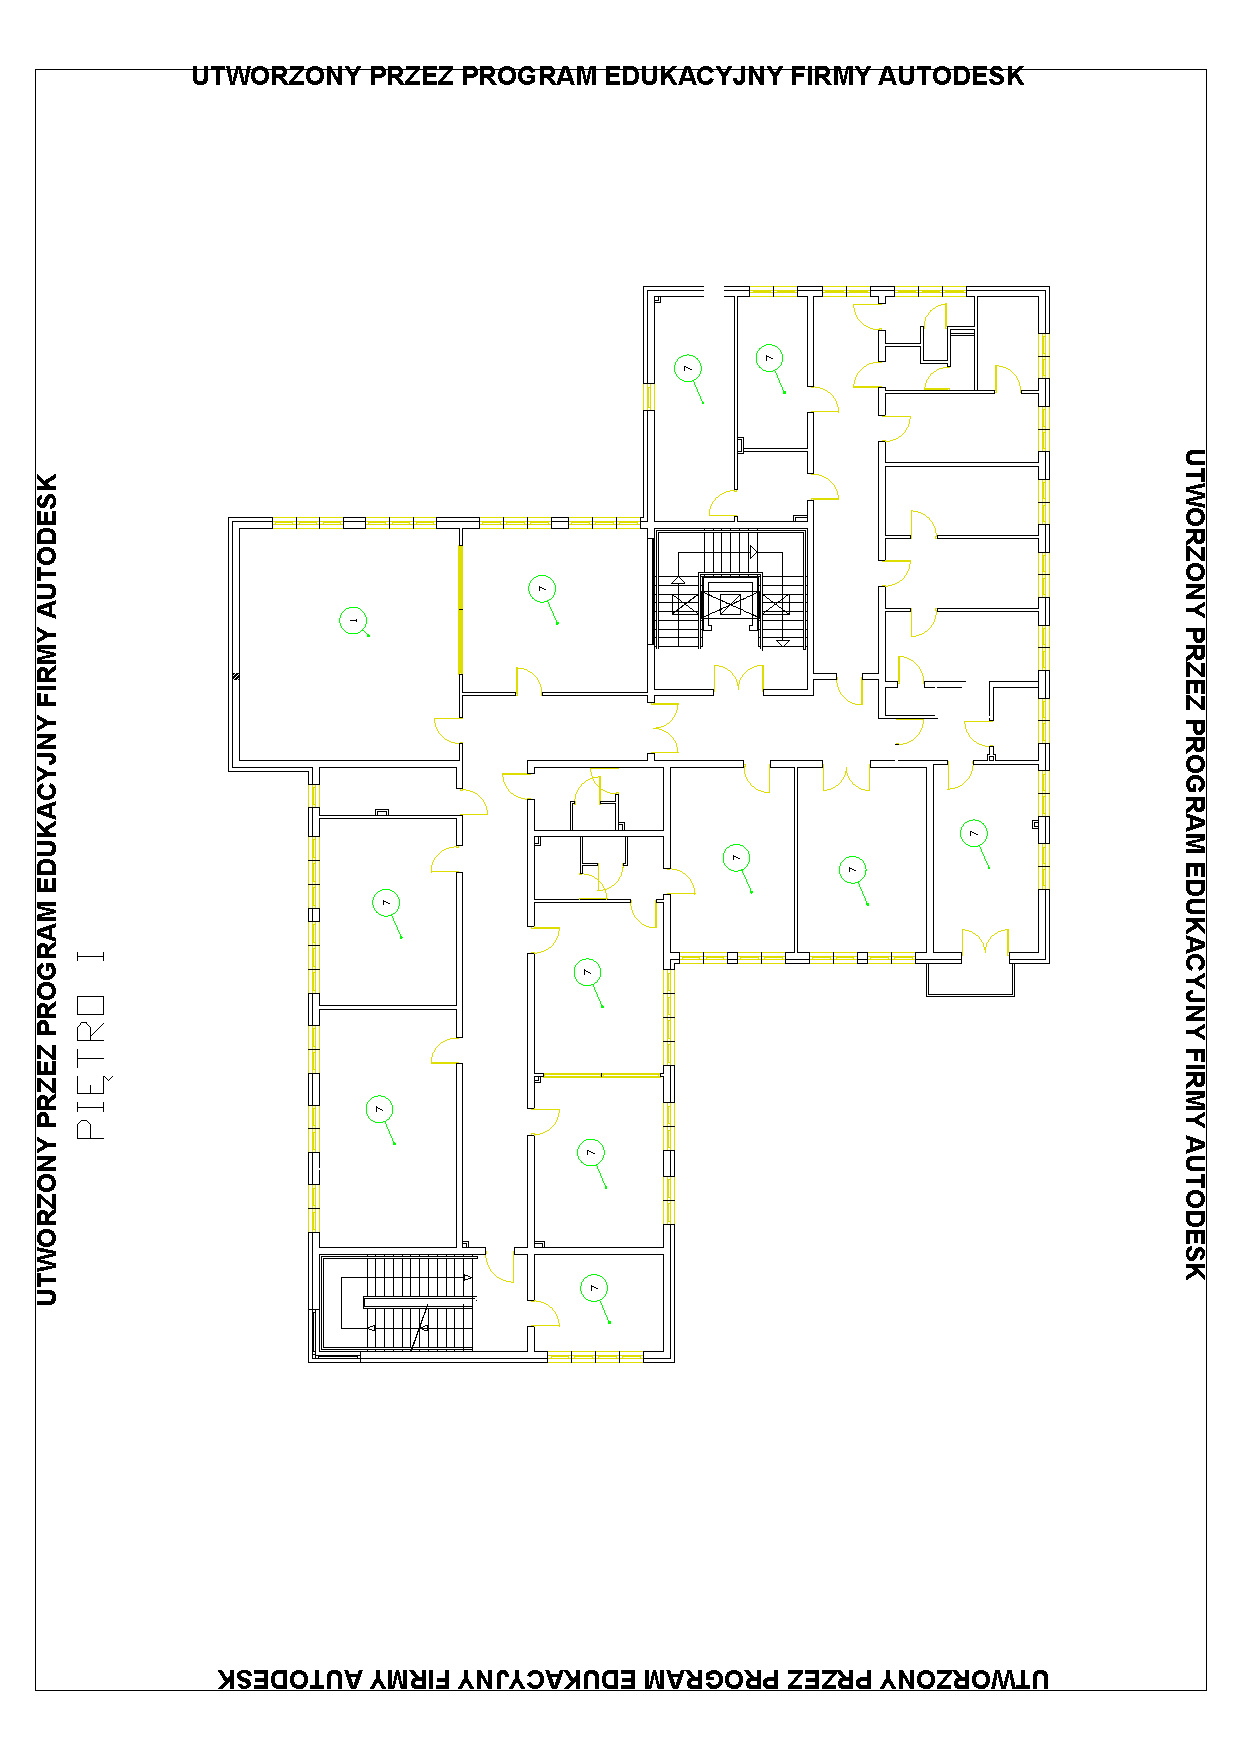
\includegraphics[width=\textwidth]{img/b2-1.pdf}
    \caption{Budynek 2 - Piętro I}
  \end{center}
\end{figure}

\begin{figure}[H]
  \begin{center}
    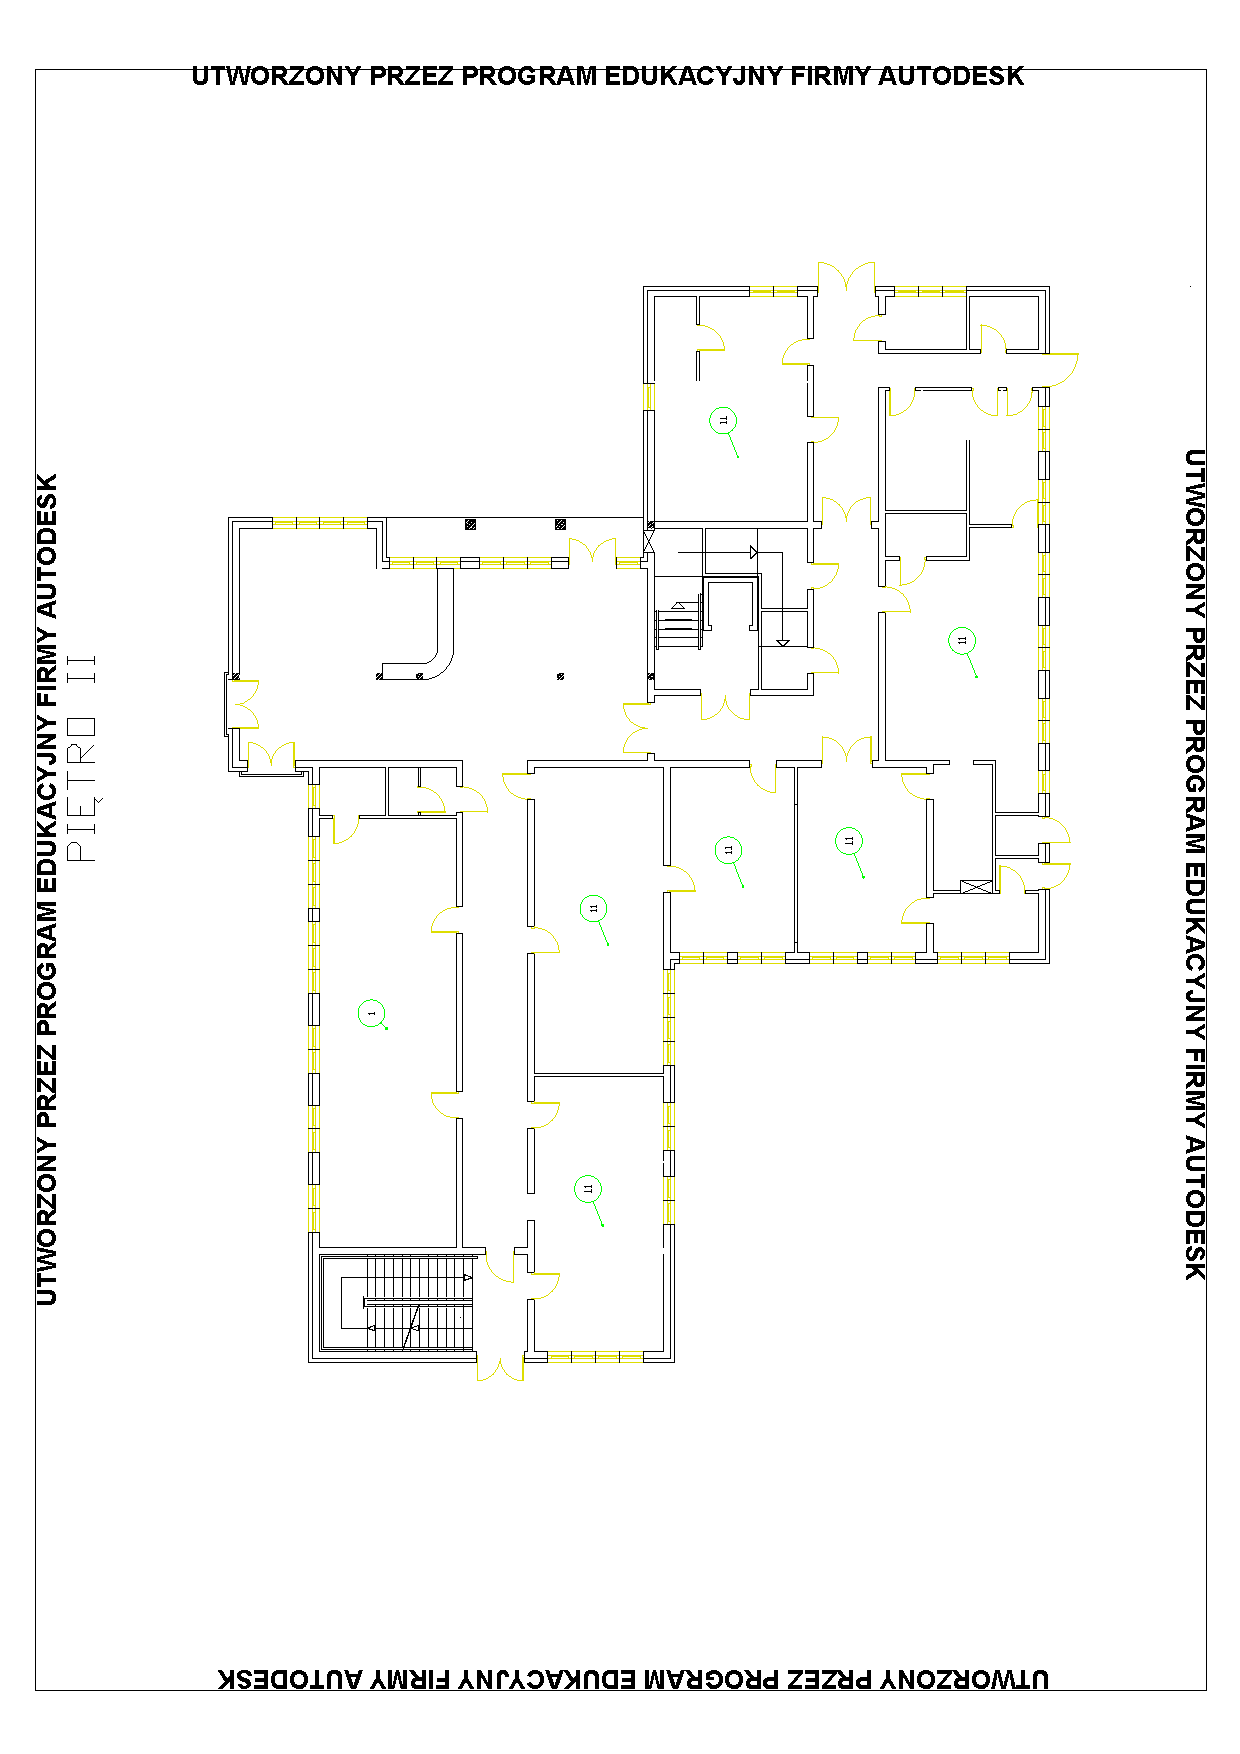
\includegraphics[width=\textwidth]{img/b2-2.pdf}
    \caption{Budynek 2 - Piętro II}
  \end{center}
\end{figure}


\newpage





\subsection{Wyposażenie}
\paragraph{}
Wyposażeniem każdego pracownika jest stacjonarny zestaw komputerowy, w skład którego wchodzą: jednostka centralna, mysz, klawiatura, monitor, kamera internetowa, słuchawki z mikrofonem.
Na każdym piętrze znajduje się sieciowe urządzenie wielofunkcyjne, podłączone i skonfigurowane w sposób zapewniający dostęp wszystkim pracownikom z danego piętra.

\paragraph{}
Każda z sal konferencyjnych została wyposażona w rzutnik multimedialny, a także komputer stacjonarny umożliwiający prowadzenie tele i wideokonferencji.
Ponadto w każdej z sal konferencyjnych umieszczony jest punkt dostępowy sieci bezprzewodowej.

\paragraph{}
Część parteru jednego z budynków została zaadaptowana jako serwerownia, w której umieszczono kilka serwerów. Serwery te pozwalają na przechowywanie repozytowiów kodu źródłowego, przprowadzanie testów oprogramowania, składownie i wymianę plików między pracownikami, kopie zapasowe danych, a także dostęp do baz danych wykorzystywanych do administracji oraz przy pracy nad projektami.

\paragraph{}
Systemy operacyjne dostępne dla pracowników:
\begin{itemize}
  \item Windows 7
  \item Ubuntu 11
  \item Mac OS X Lion 10.7
\end{itemize}

\paragraph{}
Oprogramowanie wykorzystywane przez pracowników:
\begin{itemize}
  \item Komunikator internetowy (protokół XMPP)
  \item Program do tele i videokonferencji Skype
  \item Pogram pocztowy (dowolny)
  \item System kontroli wersji (svn, git)
  \item Oprogramowanie umożliwiające współdzielenie plików Samba
  \item Narzędzia służące do wytwarzania oprogramowania :
  \begin{itemize}
	\item Windows : Microsoft Visual Studio 2010, Eclipse
	\item Linux : Eclipse
	\item Mac OS X : XCode
  \end{itemize}
  \item Program do pracy zdalnej TeamViewer
 \item Pakiet Office
\end{itemize}






